\documentclass[serif]{beamer}
\usetheme{Frankfurt}
\usecolortheme{crane}
\usefonttheme{structuresmallcapsserif}

\usepackage{tikz}
\usetikzlibrary{shapes.geometric, arrows,chains}

\tikzset{
  startstop/.style={
    rectangle, 
    rounded corners,
    minimum width=3cm, 
    minimum height=1cm,
    align=center, 
    draw=black, 
    fill=red!30
    },
  process/.style={
    rectangle, 
    minimum width=3cm, 
    minimum height=1cm, 
    align=center, 
    draw=black, 
    fill=blue!30
    },
  decision/.style={
    rectangle, 
    minimum width=3cm, 
    minimum height=1cm, align=center, 
    draw=black, 
    fill=green!30
    },
  arrow/.style={thick,->,>=stealth},
  dec/.style={
    ellipse, 
    align=center, 
    draw=black, 
    fill=green!30
    },
}

\title{Cat or Dog: Predictive Modeling}
\subtitle{STAT GU4243 - Applied Data Science}
\author{Group 6}
\institute{Columbia University}
\date{\today}

\begin{document}

\frame{\titlepage}

\section{Outline}
\frame{\tableofcontents}

\section{Introduction}
\subsection{Us}
\frame{
	\frametitle{Group members}
	Wanting Cheng, Mingkai Deng, Jiongjiong Li, Kai Li, Daniel Parker
}
\subsection{Motivation}
\frame{
	\frametitle{Why do this?---Motivation}
	\includegraphics[width=\linewidth, height=\textheight,keepaspectratio]{../../../../../Downloads/pet47.jpg}
}
\frame{
	\frametitle{Why do this?---Motivation}
	\includegraphics[width=\linewidth, height=\textheight,keepaspectratio]{../../../../../Downloads/pet197.jpg}
}

\subsection{Scope}
\frame{
	\frametitle{Spec \& Scope}
	[C]\textit{arry out model evaluation and selection for predictive analytics on image data}
	$\ldots$
	[using] \textit{a set of 4387 labeled images of cats and dogs}
	$\ldots$
	\textit{creat}[e] \textit{a mobile AI program that accurately distinguishes between} [them]
	$\ldots$
	\textit{balance between the complexity of variables/features/models used and the predictive performance.}
}
\frame{
	\frametitle{Spec \& Scope}	
	\includegraphics[width=\linewidth, height=\textheight,keepaspectratio]{../../../../../Downloads/predictiveprogram.png}
}

\section{Method}
\subsection{Exploratory analysis}
\frame{
	\frametitle{Exploratory Analysis}
	What makes one animal different from another?
	[Intuition]
	
	What approaches did previous semesters' groups employ?
	[Research]
}

\subsection{Feature extraction}
\frame{
	\frametitle{Feature Extraction}
	\begin{enumerate}
	\item<1-> SIFT = scale-invariant feature transformation.
	\item<2-> HOG = histogram of oriented gradients.
	\item<3-> LBP = local binary patterns.
	\item<4-> HSV = hue, saturation, value.
	\item<5-> RGB = red, green, blue.
	\end{enumerate}
}
\subsection{Statistical machine learning models}
\frame{
	\frametitle{Statistical Machine Learning Models}
	\begin{enumerate}
	\item<1-> Gradient boosting machine---the baseline.
	\item<2-> Random forests.
	\item<3-> TensorFlow/Keras neural network.
	\item<4-> Support vector machine.
	\item<5-> Adaptive boosting (``AdaBoost").
	\item<6-> Extreme gradient boosting (``XGBoost").

	\end{enumerate}}

\subsection{Tuning and training}
\frame{
	\frametitle{Tuning and Training}
	Simplifying heuristic: use \textit{all} features, rather than subsets.
		
	Preference for built-in package functions, rather than a generalized syntax.
}
\frame{
	\frametitle{How we finalized models---Flowchart}
	\centering
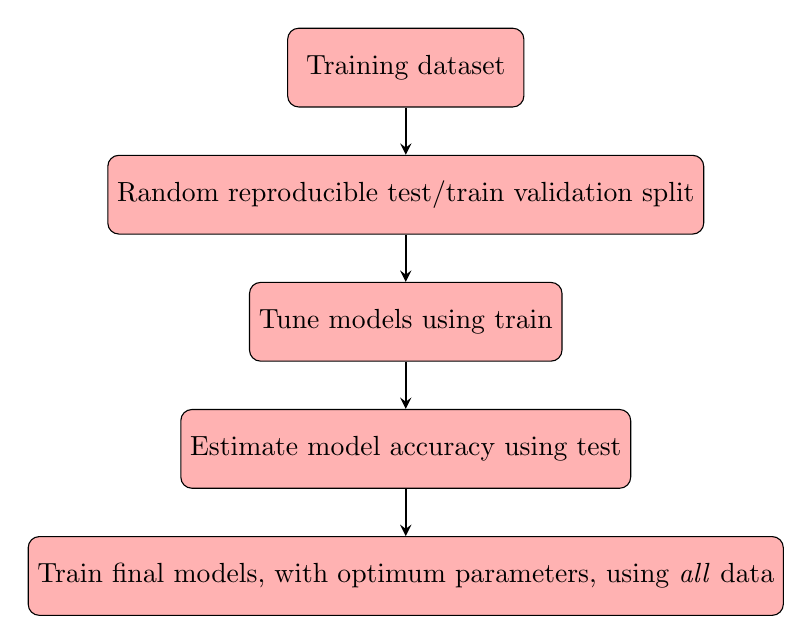
\begin{tikzpicture}[
  start chain=going below,
  every join/.style={arrow},
  node distance=0.6cm
  ]
\node (step1) [startstop,on chain,join] {Training dataset};
\node (step2) [startstop,on chain,join] {Random reproducible test/train validation split};
\node (step3) [startstop,on chain,join] {Tune models using train};
\node (step4) [startstop,on chain,join] {Estimate model accuracy using test};
\node (step5) [startstop,on chain,join] {Train final models, with optimum parameters, using \textit{all} data};
\end{tikzpicture}	
}
\section{Results}
\frame{
	\includegraphics[width=\linewidth, height=\textheight,keepaspectratio]{../../../../../Downloads/predictiveprogram.png}
}
\frame{
	\frametitle{Training Cost}
	Computation time and memory use for:
	1. Feature extraction
	2. Model training
% Table including the information that's been determined
}

\frame{
	\frametitle{Test / Use Cost}
	Computation time for:
	1. Feature extraction 
	2. Classification
% Table including the information that's been determined
}

\frame{
	\frametitle{Accuracy}
% Table including the information that's been determined
}
\frame{
	\frametitle{Comparison}
% ggplot visualization scatterplot: 
%% x axis: time to make prediction
%% y axis: accuracy in percentage
}

\section{Discussion}
\frame{
	\frametitle{Further directions to explore}
	\begin{enumerate}
	\item<1-> Other extractions and combinations thereof.
	\item<2-> Dataset manipulation to ``grow" more training data for free.
	\item<3-> Other models.
	\item<4-> Ensembling.
	\item<5-> $\ldots$
	\end{enumerate}
}
\frame{
Thank you!
}

\end{document}